\section{Methods}

To archive clustering, the method adopted was to compare document using the authorship linkings strategies presented in \textit{Evaluation of text representation schemes and distance measures for authorship linking} \cite{kocher_verification}.
In this paper the authors compare multiple text representation based on author style which correspond to : words frequencies, lemma frequencies, Part-Of-Speach (POS) tags frequencies, short sequences of POS tags, as well as n-grams frequencies.
The distance mesures used are : $L^1$ norms (Manhattan, Tanimoto), $L^2$ norm (Matusita, Clark), inner products (Cosine distance) and the Jeffery divergence.
Depending on the dataset, the text representation and the metric used, no clear text representation and different distance mesures were giving better or worse results.

In this study to archive a good clustering, the main objective is to have a reliable authorship linking rank list.
To try to increase the quality of the rank list, the proposed method is to use a combination of multiple rank list using different strategies to form a optimistically better rank list.
By using the most diverse strategies, we belive it is possible to increase the quality using the principle of combinaison of evidences.

\subsection{Feature vectors}

To be able to express a document as a feature vector of size N the common stragegy in Stylometry is to find the N most frequant words (N-MFW) in a corpus, and for each document compute the relative frequancy of each of these words for the document \cite{savoy_stylo}.
For example if the word : "\textit{the}" is in the N-MFW and occure 50 times in a document with 300 words, its relative frequancy is $50/300 = 1/6$, which will be one of the composante of the feature vector.
No clear value of N for the N-MFW is to choose over others, but a value between 50-500 tends to produce good results \cite{savoy_text_representation}.

Instead of using directly the words to create the feature vector, another possibility is to use the lemma corresponding to each words, for example the stentence \textit{I saw two men with a saw} its lematized version is : \textit{I see two man with a saw} this require advanced text pre-processing but it can remove ambiguity.

Another popular method is instead of considering every token as a word, this method aim to create a "word" from short a sequences of letters called n-grams using Definition~\ref{def:n-grams}.
To consider overlapping word, the whole document is synthetized into a long string by joining every token by a \textit{underscore} : $\_$.
This technique can be further exploited by combining for example two or more sizes of n-grams together.
N-grams can be really effective even though no clear meaning from each n-grams can be exploited at first sight, but by using n-grams of size 3 to 5 in most germanic languages this can correspond to for example the tense of the verbs (i.e. : \textit{ing\_}, \textit{ed\_}), some small common words (\textit{\_the\_}, \textit{\_and\_}, \textit{\_that}), or for example to adverbs in French (\textit{\_ment}), etc.

\begin{definition}[$n$-grams]
  \label{def:n-grams}
  A $N$-gram is a special type of tokenization which is constructed by creating a token of size $N$ for each substrings starting from the position $0$ to \textit{text\_size} - $N$.
  Example: Using 3-grams The string: "brown fox" is converted to: \\
  $("\text{bro}", "\text{row}", "\text{own}", "\text{wn\_}", "\text{n\_f}", "\text{\_fo}", "\text{fox}")$
\end{definition}

Another possible stylistic aspect that can be detected from a text is to consider the sentence constructions.
This can be solved by creating short sequences (n-grams) of POS tags.
In this case, we consider each POS as a character in the n-grams definition, this is also known as w-shingling.
For example, the sentence : \textit{"The cat eat a fish"} has the following POS tag \textit{"Article Noun Verb Article Noun"} which correspond to the following 3-grams of POS : \textit{"Article Noun Verb"} / \textit{"Noun Verb Article"} / \textit{"Verb Article Noun"}.
In practice the POS is more detailed, for example instead of just considering the verb, the verb and its tense can be used, the same goes for the other type of POS.

\subsection{Smoothing}

When considering relative term frequcencies they can be used as a probability of occurance by using the maximum likelihood principle.
The main problem with this approach is that we tends to overhistimate the probability of occurance of frequant terms and underhestimate the probability of ocucrance of low frequcency terms, for example if a word is not found in a document this doesn't mean the probability of the author using this word is 0.
The solution proposed is to use smoothing, such as the Lidstone smoothing presented in Definition~\ref{def:lidstone_smoothing}.
Smoothing techniques can help distance functions based on probabilities, such as the Kullback-Leibler Divergence.

\begin{definition}[Lidstone smoothing \cite{savoy_stylo}]
  \label{def:lidstone_smoothing}
  \begin{equation}
    p(t_i, D_j) = \frac{tf_{i,j} + \lambda}{n + \lambda \cdot |V|}
  \end{equation}
  With $t_i$ the i-th term, $D_j$ the j-th document, $tf_{i,j}$ the number of occurance of the i-th term in $D_j$, $|V|$ the size of the vocabulary, $\lambda$ a small value ($\lambda = 1$ special, case called Lalpace smoothing, but generally a smaller value such as 0.1 give good results), n the total number of words in the document $D_j$
\end{definition}

\subsection{Vectors distances and normalization}

\begin{definition}[Manhanttan distance ($L^1$ based)]
  To compute the Manhanttan distance the following equation is used.
  \begin{equation}
    dist_{Manhanttan}(A, B) = \sum_{i=1}^{m} |A_i - B_i|
  \end{equation}
\end{definition}

\begin{definition}[Tanimoto distance ($L^1$ based, normalized)]
  To compute the Tanimoto distance the following equation is used. It's a components-wised normalized version of the manhattan distance.
  \begin{equation}
    dist_{Tanimoto}(A, B) = \frac{dist_{Manhattan}(A, B)}{\sum_{i=1}^{m} max(A_i, B_i)}
  \end{equation}
\end{definition}

\begin{definition}[Euclidean distance ($L^2$ based)]
  To compute the Euclidean distance the following equation is used.
  \begin{equation}
    dist_{Euclidian}(A, B) = \sqrt{\sum_{i=0}^{m}(A_i - B_i)^2}
  \end{equation}
\end{definition}

\begin{definition}[Matusita distance ($L^2$ based, square rooted values)]
  To compute the Matusita distance the following equation is used.
  \begin{equation}
    \begin{split}
      dist_{Matusita}(A, B) &= dist_{Euclidian}(A', B') \\
      \text{with }A' &= \sqrt{A}\text{ and }B' = \sqrt{B}
    \end{split}
  \end{equation}
\end{definition}

\begin{definition}[Clark distance ($L^2$ based)]
  To compute the Clark distance the following equation is used.
  \begin{equation}
    dist_{Clark}(A, B) = \sqrt{\sum_{i=0}^{m}\left(\frac{|A_i - B_i|}{A_i + B_i}\right)^2}
  \end{equation}
\end{definition}

\begin{definition}[Cosine distance (Inner product based)]
  To compute the Cosine distance to first the Cosine similarity to compote the cosine distance.
  \begin{equation}
    sim_{Cosine}(A, B) = \frac{A \cdot B}{\sqrt{A \cdot A}\sqrt{B \cdot B}}
  \end{equation}
  \begin{equation}
    dist_{Cosine}(A, B) = 1 - sim_{Cosine}(A, B)
  \end{equation}
  \begin{equation}
    angular_dist_{Cosine}(A, B) = \frac{cos^{-1}sim_{Cosine}(A, B)}{\pi}
  \end{equation}
\end{definition}

\begin{definition}[Z-score normalization \cite{savoy_stylo}]
  \begin{equation}
    Z-score(A) = \frac{A - \mu}{\sigma}
  \end{equation}
  When using the z-score normalization on MFW vectors, $\mu$ and $\sigma$ usually are vectors containing the mean and the standard deviation of each terms in the corpus.
  The Manhattan distance applied on a Z-score normalized MFW vector is also called Burrows's Delta~\cite{savoy_stylo}.
\end{definition}


\subsubsection{POS n-grams}

Figure~\ref{fig:pos_ngrams} show the average precision on the rank list produced by using POS n-grams over the number of MFW (most frequent word, in this case POS n-grams are considered as words).
The two following informations can be intuitively observed on this plot:

A more complex POS n-gram requirement more MFW to archive its maximal effectiveness.
In the St-Jean corpus 26 POS are used to describe every words in the corpus.
Which correspond to $26^2 = 676$ possible unique POS 2-grams, to $26^3 = 17'576$ POS 3-grams and $26^4 = 456'976$.

Like the other methods, an overfit to less important words is possible if the MFW ceiling is too high, reducing the average precision.
In Figure~\ref{fig:pos_ngrams} the POS 2-grams clearly have drop in average precision after \~250-MFW.

\begin{figure}
  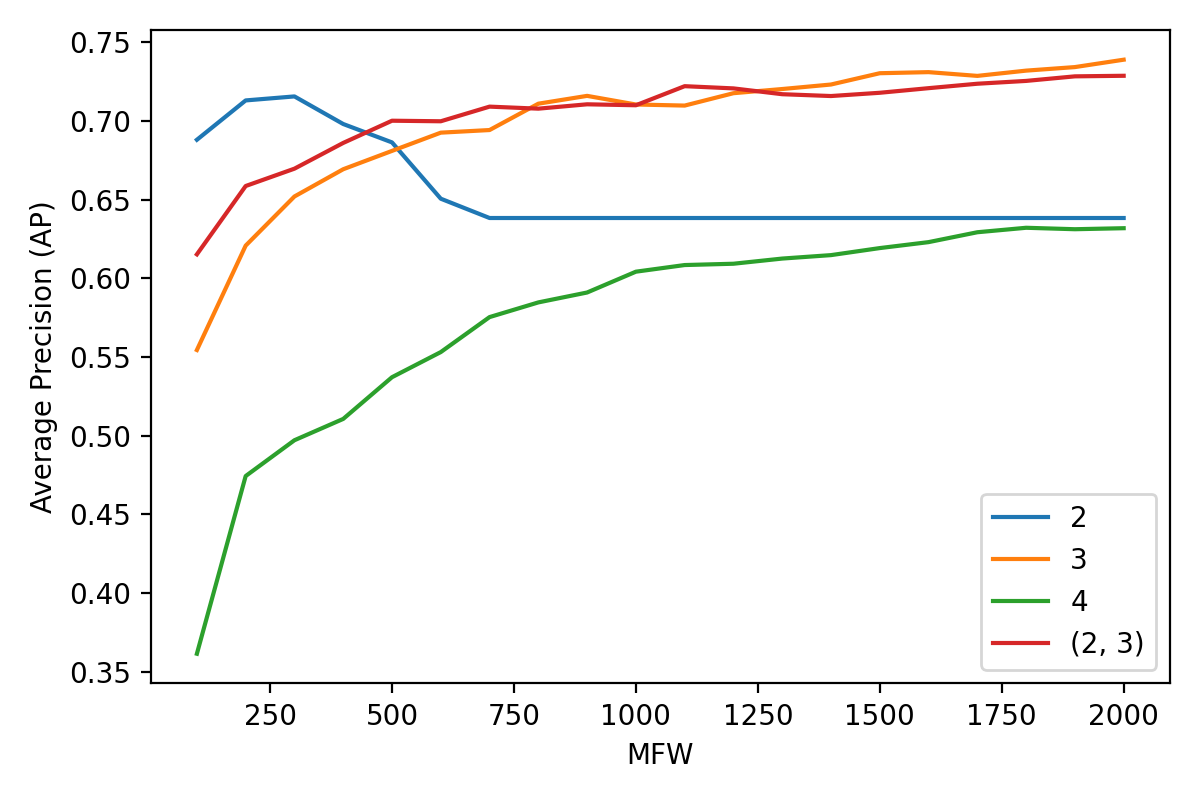
\includegraphics[width=\linewidth]{img/pos_ngrams.png}
  \caption{Average precision over the MFW in the rank list generated using the z-score normalized cosine distance.}
  \label{fig:pos_ngrams}
\end{figure}

\subsubsection{First letters, last letters of tokens}

With this methods, the goal is to extract the N first letter of each word tokens which correspond generaly to the meaning of a word.
This approach is closely related to the lemma approach.
Extract also the N last letter of each word tokens which in this case correspond to the role of the word in a sentence.
This second approach is closely related to the POS approach.

These two methods can be considered as simplified n-grams approach of the same size.

Figure~\ref{fig:first_last_letters_ngrams} shows the average precision using the z-normalized cosine distance on the experiment for N = 4.

\begin{figure}
  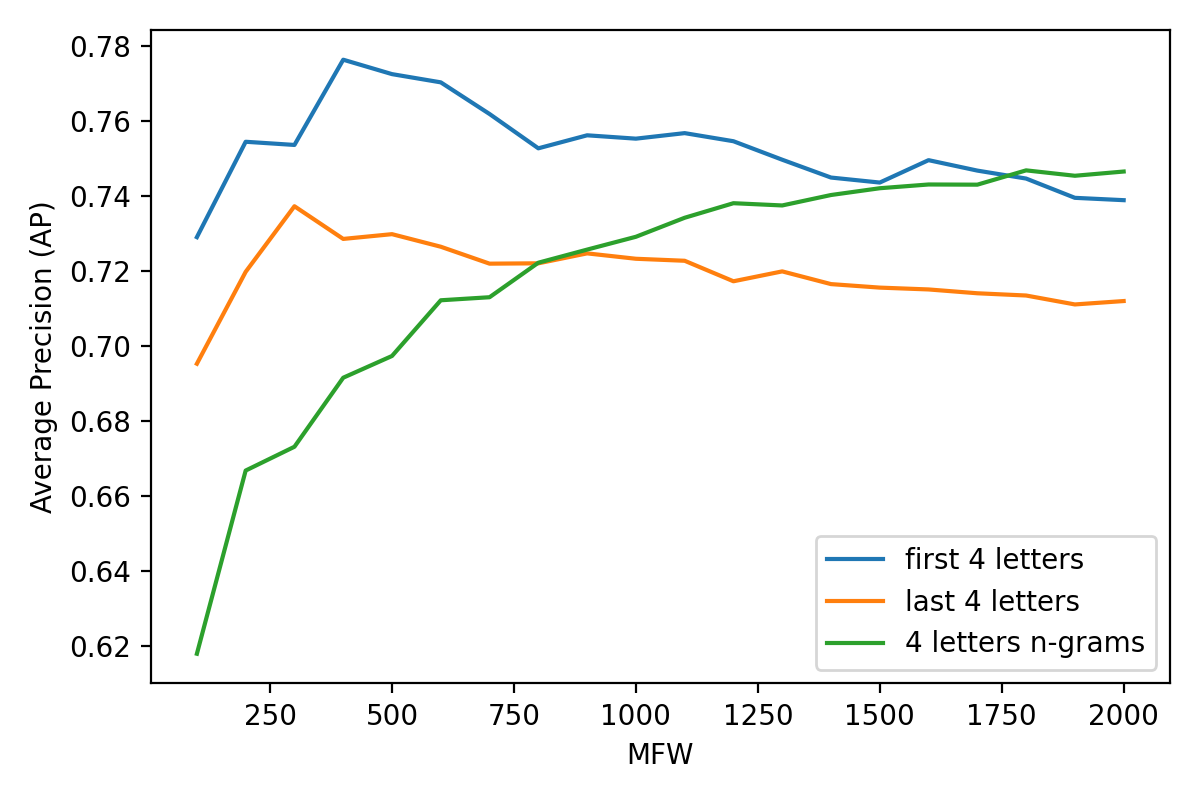
\includegraphics[width=\linewidth]{img/first_last_letters_ngrams.png}
  \caption{Average precision over the MFW in the rank list generated using the z-score normalized cosine distance.}
  \label{fig:first_last_letters_ngrams}
\end{figure}

\subsection{Compression-based distances}

This section covers the compression based strategy to compute a distance between two documents.
The main idea is to compress two documents A, B, compress the string concatenation AB of A, B and compare their sizes after compression using one of the distance mesure demonstrated below, and a lossless compression algorithm such as the Lempel-Ziv family (GZIP), block sorting family (BZip2), statistical family (PPM)~\cite{comparing_compression}.
This technique is based on the fact that compressing algorithm tries to lower the Shannon entropy of a document, thus when compressing a document with a large Shannon entropy the compressed document should have a larger size after compression than to a document with a small Shannon entropy.
Thus when concatenating two documents with a lot in common, the entropy of the concatenated document should be lower than if the two documents are very different.

\begin{definition}[Normalized compression distance \cite{savoy_stylo} \cite{comparing_compression}]
  The normalized compression distance of two documents A and B using the size after compression C is computed as follow:
  \begin{equation}
    NCD(A, B) = \frac{C(AB) - \min(C(A), C(B))}{\max(C(A), C(B))}
  \end{equation}
  Give a value in $\left[0-1+\epsilon\right]$, with $\epsilon$ being a small positive value created by the imperfection of compression algorithms).
\end{definition}

\begin{definition}[Conditional complexity of compression]
  The conditional complexity of compression of two documents A and B using the size after compression C is computed as follow:
  \begin{equation}
    CCC(A, B) = C(AB) - C(A)
  \end{equation}

\end{definition}

\begin{definition}[Compression-based cosine]
  The compression-based cosine of two documents A and B using the size after compression C is computed as follow:
  \begin{equation}
    CBC(A, B) = 1 - \frac{C(A) + C(B) - C(AB)}{\sqrt{C(A) \cdot C(B)}}
  \end{equation}
\end{definition}

\subsubsection{Rank list fusion}

Each rank list is ordered by a score, this score depend on distance measure used, thus the order of magnitude of each rank list is different.
To avoid having to problems in merging rank list with different magnitude, the solution opted is to only use the rank of each link.

An additional constraint desired is to favor top ranked link and penalize bottom ranked links when fusing rank lists.
This constraint can be easily explained by observing the distance over the rank graph of the rank list.
Figure~\ref{fig:distance_over_rank} clearly show us the top ranked links and bottom ranked links have a more sharper decision than in than the middle section.

\begin{figure}
  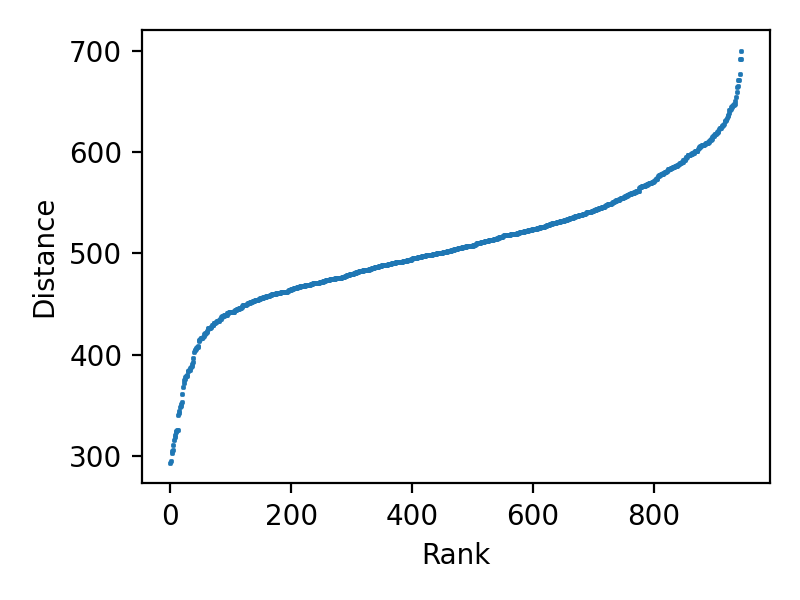
\includegraphics[width=\linewidth]{img/distance_over_rank.png}
  \caption{Distance over rank in the links of the Brunet dataset using Manhattan distances using the 500 most frequent tokens.}
  \label{fig:distance_over_rank}
\end{figure}

Top ranked links correspond to similar documents and bottom links correspond to negatively correlated documents.
Assuming that the top rank are true links after the rank list fusion these link should also be top rank.
The same reasoning can be apply for the bottom links by assuming them as false links.
A weighting curve must be design accordingly.
Using the reciprocal of the sigmoid function we can modelize such curve.
Sigmoid functions presented in Equation~\ref{eq:sigmoid} and Figure~\ref{fig:sigmoid}.
It's reciprocal in Equation~\ref{eq:sigmoid_r} and Figure~\ref{fig:sigmoid_r}.

\begin{equation}
  \label{eq:sigmoid}
  S(x) = \frac{1}{1+e^-x}
\end{equation}
\begin{equation}
  \label{eq:sigmoid_r}
  S^{-1}(x) = -\ln{\frac{x-1}{x}}
\end{equation}

\begin{figure}
  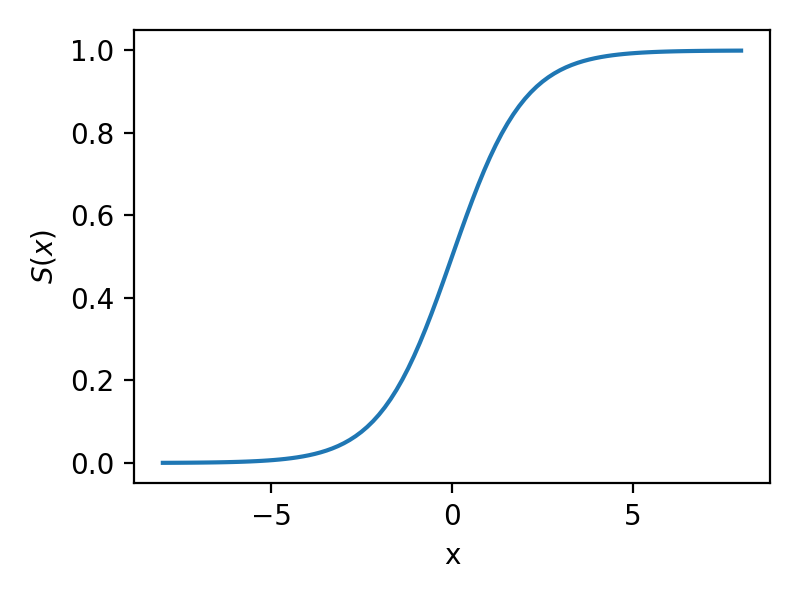
\includegraphics[width=\linewidth]{img/sigmoid.png}
  \caption{Sigmoid function between -4 and 4}
  \label{fig:sigmoid}
\end{figure}
\begin{figure}
  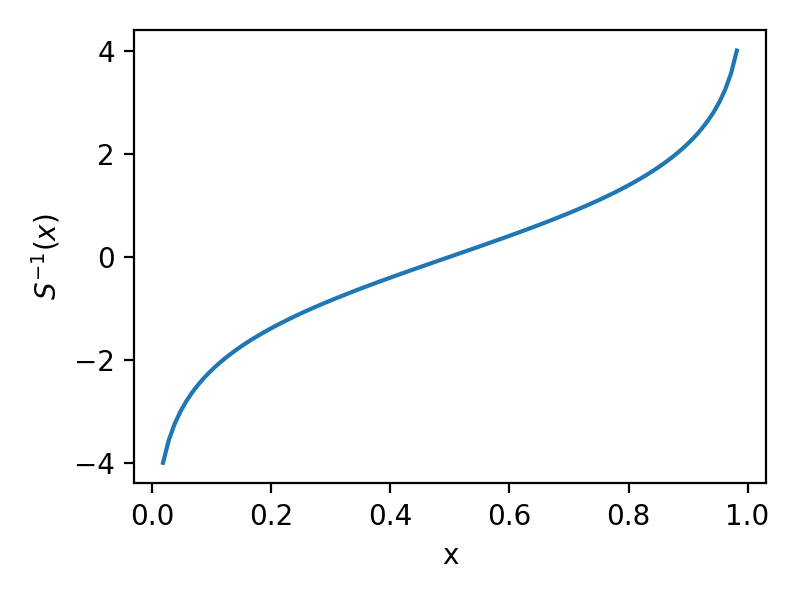
\includegraphics[width=\linewidth]{img/sigmoid_r.png}
  \caption{Reciprocal of the sigmoid function between sigmoid(-4) and sigmoid(4)}
  \label{fig:sigmoid_r}
\end{figure}

The steepness of the curve can be ajusted by changing the start and the end of the interval and then normalizing the values between 0 and 1. Figure~\ref{fig:s_curve_c} shows the $S^-1(x)$ function for the intervals between $\left[\lim\limits_{x \rightarrow 0}S(x), \lim\limits_{x \rightarrow 0}S(x)\right]$ and $\left[S(-20), S(+20)\right]$. The interval $\left[S(-4), S(+4)\right]$ correspond to Figure~\ref{fig:sigmoid_r}.
A greater interval size increase the steepness which correspond to an increase of the rank conservation of the top and bottom ranked links and decreasing the rank conservation of the middle ranked links.

\begin{figure}
  \centering
  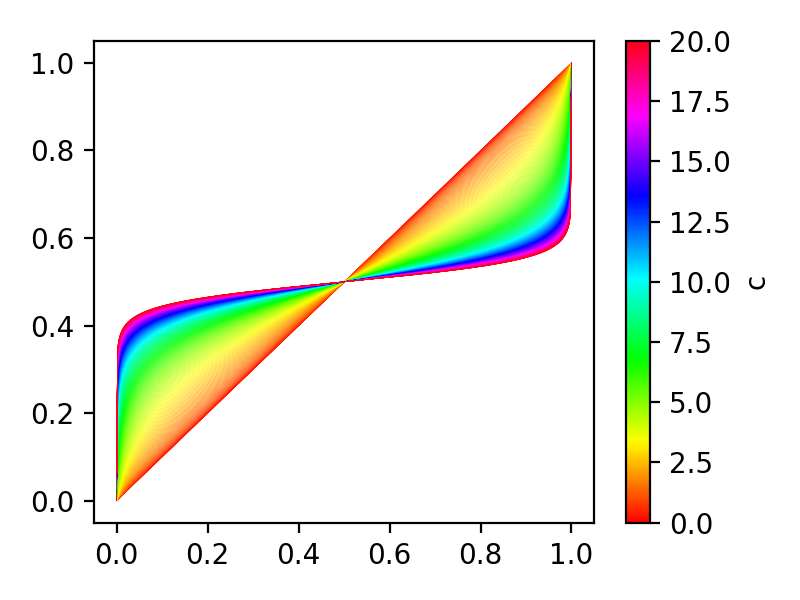
\includegraphics[width=\linewidth]{img/s_curve_c.png}
  \caption{$S^-1(x)$, sampled in $\left[S(-c), S(+c)\right]$ and normalized between 0 and 1}
  \label{fig:s_curve_c}
\end{figure}

To break the symmetry for the curve, to be able increase the conservation of the top rank while decreasing the conservation of the bottom ranked. The solution proposed is to take $r \cdot N$ samples for $\left[S(-c), S(0)\right]$ and $(1-r) \cdot N$ samples for $\left[S(0), S(c)\right]$. Figure~\ref{fig:s_curve_r} shows $\left[S(-4), S(4)\right]$ with $r \in \{0.25, 0.5, 0.75\}$.

\begin{figure}
  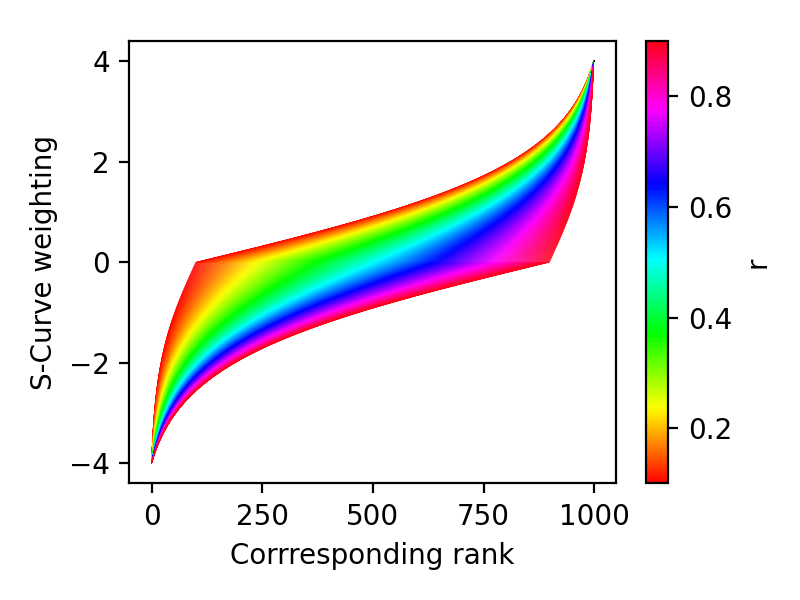
\includegraphics[width=\linewidth]{img/s_curve_r.png}
  \caption{Sampling $S^-1(x)$ with $r \cdot N$ samples for $\left[S(-c), S(0)\right]$ and $(1-r) \cdot N$ samples for $\left[S(0), S(c)\right]$}
  \label{fig:s_curve_r}
\end{figure}


\subsection{Authors Clustering}

To find clusters of authors, a possible way is to use a hierarchical clustering algorithm on a rank list.
In a rank list, each link indicate that both documents should belong to the same cluster in order of certainty.
The hardest task in this clustering scheme is to find the right cut in the rank list.
This cut should maximize the number of true links above the cut and the number of false links under the cut.
To find this cut, two apporaches were explored : one using a unsupervised clustering evaluation technique which is totaly unsupervised and another one using a linear model to learn to make this cut but it requires a training dataset.

\subsubsection{Agglomerative clustering}

The scikit-learn package~\cite{sklearn} provide an implementation bottom-up implementation of the hierarchical clustering, which is usually called agglomerative clustering.
Using this approach, at the start of the algorithm, each document belong to a different cluster.
Clusters are merge based on the scores in the rank list, each step the algorithm merge clusters using the minimal score based on the linkage criteria.
Multiple linkage criteria are available : \textit{ward} (metric that aim to minimize the variance of the cluster merged), \textit{average-linkage} (use the average score of each links of the cluster merged), \textit{complete-linkage} (use the maximal score of the cluster merged), \textit{single-linkage} (use the minimal score of the cluster merged).
Ward linkage was discarded since the implementation only allow euclidean distance for its computation.

\subsubsection{Learning the cut in a unsupervised way}

The silhouette score is a unsupervised clustering metric which evaluate a clustering result by mesureing the cohesion and separation of the clusters.
A large value indicate a good cohesion and good separation of the clusters.
Running the agglomerative clustering at each cut in the rank list then evaluating the clustering result using the silhouette score, the maximal shilhouette score position give a good indication where the best cut is.

\subsubsection{Learning the cut in a supervised way}



\subsection{Complexity}
